\chapter{四季中的动物}\label{ch:g3:animals-through-seasons}

十月里，燕子成排停在电线上，某个早晨，
它们便不见了踪影。篱笆下的刺猬把自己蜷进
树叶窝里，要到春天才会再露面。狐狸
则在每场大雪中照常外出。冬天是艰难的季节——
寒冷，尤其是食物匮乏——\omterm{def:g1:animals-around-us:animal}{动物}有三种
重要的办法熬过冬天。

\section{冬季：匮乏的季节}

\begin{proposition}[冬季的双重难题]\label{prop:g3:animals-through-seasons:problem}
冬季让\omterm{def:g1:animals-around-us:animal}{动物}同时面对两个难题：
\begin{enumerate}
  \item \emph{寒冷}，它会更快地带走体温——而
        保暖需要消耗\omterm{prop:g3:balanced-diet:jobs}{能量}
        （见\cref{prop:g3:balanced-diet:jobs}）；
  \item \emph{食物匮乏}：\omterm{def:g1:plants-around-us:plant}{植物}停止生长，\omterm{prop:g3:sorting-living-things:groups}{昆虫}
        消失，\omterm{def:g3:food-chains:chain}{食物链}的起始环节在
        \cref{ch:g3:food-chains}中变得稀少——于是
        匮乏会向上传递，波及所有\omterm{def:g1:living-or-not:living}{生物}。
\end{enumerate}
需要更多的热量，却只有更少的食物可用：这就是冬季
每种\omterm{def:g1:animals-around-us:animal}{动物}都必须解决的难题。
\end{proposition}
\admitted

\begin{example}[食虫动物的食物去哪儿了？]\label{ex:g3:animals-through-seasons:insects}
燕子以飞行中的\omterm{prop:g3:sorting-living-things:groups}{昆虫}为食，在空中捕捉。到
十一月，空中已经没有\omterm{prop:g3:sorting-living-things:groups}{昆虫}了：天气太冷。对于
专为空中捕食而生的鸟来说，改换食谱也无济于事——燕子的
食物来源会完全消失。
\end{example}

\begin{omfigure}
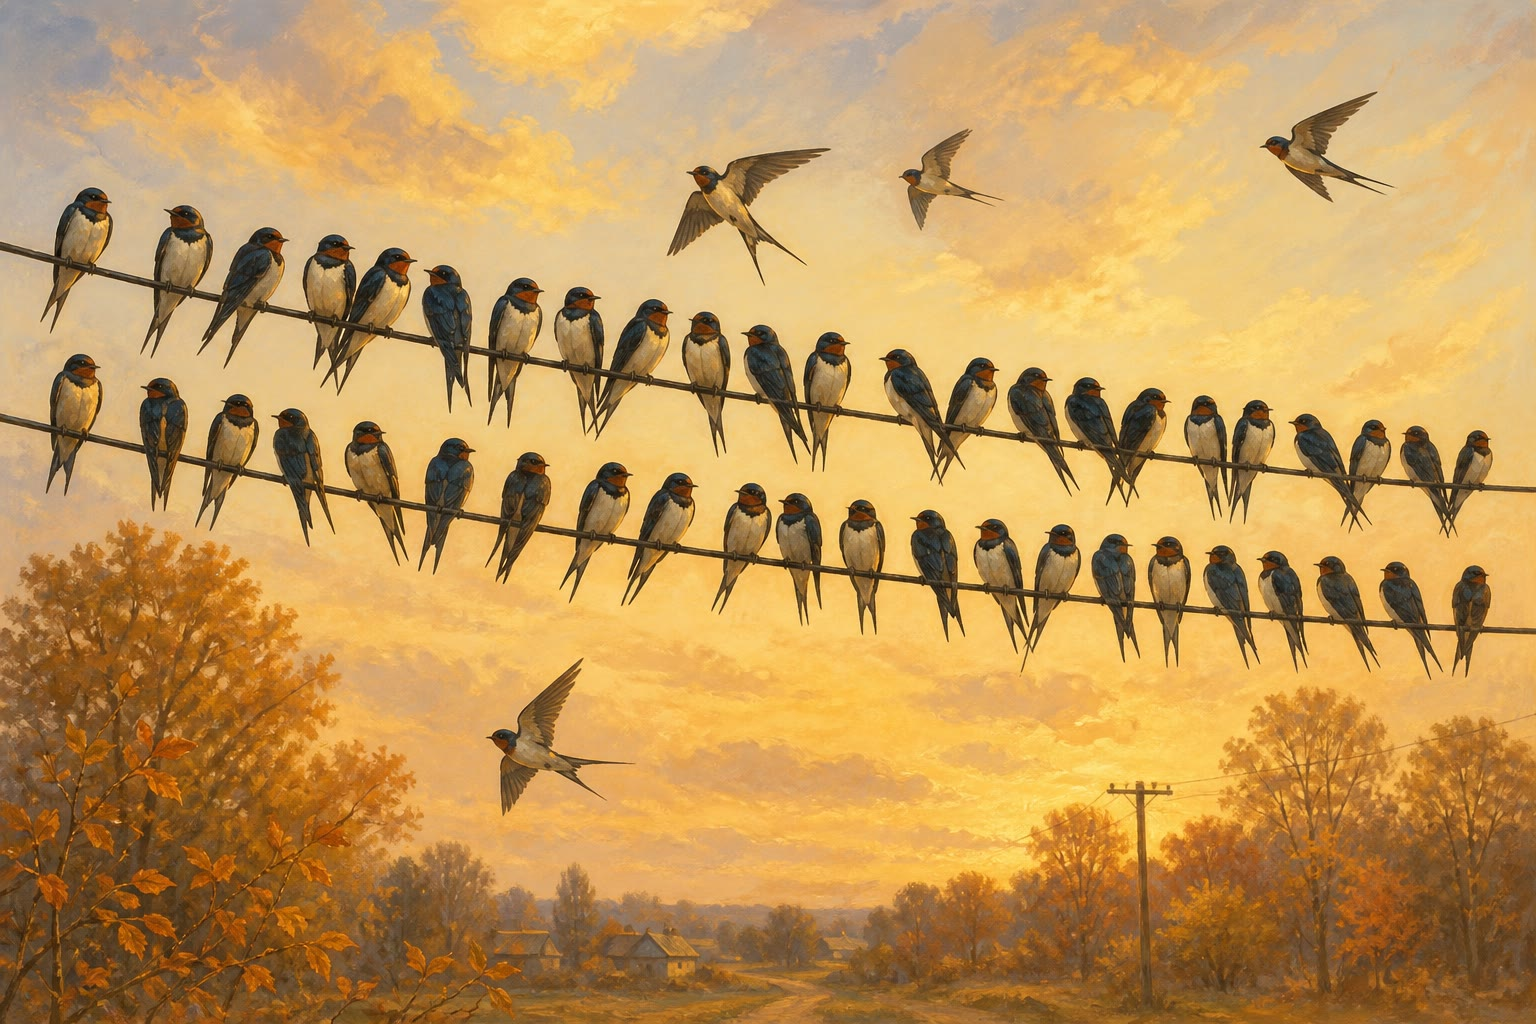
\includegraphics[width=0.62\linewidth]{images/book1/ai/g3-seasons-swallows.jpg}

{\small 十月，燕子在电线上聚集，准备
出发，距离\omterm{prop:g3:sorting-living-things:groups}{昆虫}消失只剩几天。}
\end{omfigure}

\section{应对冬季的三种办法}

\begin{definition}[迁徙]\label{def:g3:animals-through-seasons:migration}
\emph{迁徙}\index{迁徙}是指每年随季节变化，
从一个地区迁往另一个地区：在冬季来临前离开，
前往仍有食物的温暖地带，并在春季返回。
燕子、白鹳和鹤都是
\emph{迁徙动物}\index{迁徙}；有些会飞行数千
千米，并能找回原先的同一个鸟巢。
\end{definition}

\begin{definition}[冬眠]\label{def:g3:animals-through-seasons:hibernation}
\emph{冬眠}\index{冬眠}是指在隐蔽的住所里
度过冬季，陷入深沉而寒冷的\omterm{prop:g1:healthy-habits:needs}{睡眠}：体温下降，心跳
和呼吸减慢到几乎停止，\omterm{def:g1:animals-around-us:animal}{动物}慢慢依靠秋天
储存的脂肪维持生命。刺猬、睡鼠、
旱獭和蝙蝠都会冬眠。
\end{definition}

\begin{definition}[保持活动]\label{def:g3:animals-through-seasons:active}
其余\omterm{def:g1:animals-around-us:animal}{动物}\emph{保持活动}\index{保持活动（冬季）}，并改变它们的
装备或习性：更厚的
\emph{冬毛}\index{冬毛}、食物
\emph{储备}\index{食物储备}（秋天收集，
松鼠埋藏的坚果）、改换食谱
（见\cref{ex:g2:what-animals-eat:winter}中的乌鸫）、或者干脆
更费力地搜寻食物——狐狸、鹿和知更鸟。
\end{definition}

\begin{omfigure}
\begin{tikzpicture}
  \draw[thick, omDef, fill=omDef!7, rounded corners=6pt]
    (0,0) rectangle (4.1,3.1);
  \draw[thick, omProp, fill=omProp!7, rounded corners=6pt]
    (4.5,0) rectangle (8.6,3.1);
  \draw[thick, omMeth, fill=omMeth!7, rounded corners=6pt]
    (9.0,0) rectangle (13.1,3.1);
  \node[font=\small\bfseries, omDef, text height=1.6ex, text depth=0.4ex]
    at (2.05,2.75) {迁徙};
  \node[font=\small\bfseries, omProp, text height=1.6ex, text depth=0.4ex]
    at (6.55,2.75) {冬眠};
  \node[font=\small\bfseries, omMeth, text height=1.6ex, text depth=0.4ex]
    at (11.05,2.75) {保持活动};
  \node[font=\small, align=center, text width=3.8cm] at (2.05,1.2)
    {离开前往 \\ 有食物的地方 \\[2pt] 燕子、白鹳、\\ 鹤};
  \node[font=\small, align=center, text width=3.8cm] at (6.55,1.2)
    {深度寒冷睡眠 \\ 靠储存脂肪生活 \\[2pt] 刺猬、旱獭、\\ 睡鼠、蝙蝠};
  \node[font=\small, align=center, text width=3.8cm] at (11.05,1.2)
    {冬毛、储备 \\ 换食谱、努力搜寻 \\[2pt] 狐狸、松鼠、\\ 知更鸟、鹿};
\end{tikzpicture}

{\small 同一个冬天的三种应对办法。每种办法都以不同方式
解决双重难题——保暖与食物。}
\end{omfigure}

\begin{example}[三个邻居，三种策略]\label{ex:g3:animals-through-seasons:three}
一月的一片树篱里：在它上方筑过巢的燕子已
在非洲，于温暖的阳光下捕捉\omterm{prop:g3:sorting-living-things:groups}{昆虫}；树篱下的刺猬
在树叶窝里冷而缓慢地睡着，燃烧着
八月积累的脂肪；树篱顶上的知更鸟，
身披蓬松的冬羽，巡视着最后的浆果。到了四月，三者
又会在同一片树篱中忙碌起来。
\end{example}

\begin{remark}[睡眠不是懒惰，迁徙不是旅游]\label{rem:g3:animals-through-seasons:cost}
每种办法都有代价。\omterm{def:g3:animals-through-seasons:migration}{迁徙动物}要冒着
耗尽体力的长途跋涉风险；\omterm{def:g3:animals-through-seasons:hibernation}{冬眠}\omterm{def:g1:animals-around-us:animal}{动物}必须
在秋天积累起每一克冬季脂肪——十一月太瘦的刺猬
将无法在春天醒来；\omterm{def:g3:animals-through-seasons:active}{保持活动}的\omterm{def:g1:animals-around-us:animal}{动物}只能赌
能否在最饥饿的几个月里找到食物。
冬天的代价，或提前付清，或在途中付清，或逐日付清。
\end{remark}

\begin{method}[猜测动物的冬季策略]\label{met:g3:animals-through-seasons:guess}
\begin{enumerate}
  \item 问问它吃什么，以及冬天这里
        是否还有这种食物；
  \item 食物完全消失（飞行\omterm{prop:g3:sorting-living-things:groups}{昆虫}、花蜜）：推测
        会\omterm{def:g3:animals-through-seasons:migration}{迁徙}或\omterm{def:g3:animals-through-seasons:hibernation}{冬眠}；
  \item 食物仍可找到（\omterm{def:g2:from-seed-to-plant:seed}{种子}、浆果、猎物）：推测会积极过冬，
        或许会长出更厚的毛或储备食物；
  \item 在秋天检查：长膘并挖洞筑巢，说明它
        会\omterm{def:g3:animals-through-seasons:hibernation}{冬眠}；成群聚集，说明它将离开。
\end{enumerate}
\end{method}

\begin{example}[春天把一切都还原]\label{ex:g3:animals-through-seasons:spring}
三月和四月，过程倒转：\omterm{prop:g3:sorting-living-things:groups}{昆虫}回来，
\omterm{def:g3:animals-through-seasons:migration}{迁徙动物}回到旧巢，\omterm{def:g3:animals-through-seasons:hibernation}{冬眠}\omterm{def:g1:animals-around-us:animal}{动物}醒来时
身形消瘦、饥肠辘辘，\omterm{def:g3:animals-through-seasons:active}{冬毛}也脱落了。季节轮转，
\omterm{def:g1:animals-around-us:animal}{动物}的日历也随之轮转——来年秋天，
燕子又会排列在电线上。
\end{example}

\section{练习}

\begin{exercise}[$\star$]\label{exo:g3:animals-through-seasons:1}
冬天给每种\omterm{def:g1:animals-around-us:animal}{动物}带来了哪两个相互关联的问题？
\end{exercise}

\begin{exercise}[$\star$]\label{exo:g3:animals-through-seasons:2}
说出三种冬季策略，并为每种策略各举两种\omterm{def:g1:animals-around-us:animal}{动物}。
\end{exercise}

\begin{exercise}[$\star$]\label{exo:g3:animals-through-seasons:3}
\omterm{def:g3:animals-through-seasons:hibernation}{冬眠}的刺猬在长时间\omterm{prop:g1:healthy-habits:needs}{睡眠}期间，身体会发生
什么变化？它靠什么维持生存？
\end{exercise}

\begin{exercise}[$\star$]\label{exo:g3:animals-through-seasons:4}
燕子究竟为什么必须离开？它吃的是什么，
而这种食物在冬天的这里会怎样？
\end{exercise}

\begin{exercise}[$\star$]\label{exo:g3:animals-through-seasons:5}
说出活动型\omterm{def:g1:animals-around-us:animal}{动物}度过冬天的三种方式，
并各举一种\omterm{def:g1:animals-around-us:animal}{动物}为例。
\end{exercise}

\begin{exercise}[$\star$]\label{exo:g3:animals-through-seasons:6}
根据
\cref{rem:g3:animals-through-seasons:cost}，每种策略各要付出什么代价？
\end{exercise}

\begin{exercise}[$\star$]\label{exo:g3:animals-through-seasons:7}
秋天，有一只\omterm{def:g1:animals-around-us:animal}{动物}被看到大量进食，并用干树叶铺垫
洞穴。它正在为哪种策略做准备？是
\cref{met:g3:animals-through-seasons:guess}中的哪一步告诉你的？
\end{exercise}

\begin{exercise}[$\star$]\label{exo:g3:animals-through-seasons:8}
试一试：在一个寒冷的星期里，记录你在户外实际看到的
\omterm{prop:g3:sorting-living-things:groups}{鸟类}，列出冬季清单。清单上有燕子吗？你看到的鸟中，
哪些选择了积极过冬的策略？
\end{exercise}

\begin{exercise}[$\star\star$]\label{exo:g3:animals-through-seasons:9}
用\cref{met:g3:animals-through-seasons:guess}分析以下两种\omterm{def:g1:animals-around-us:animal}{动物}：(a)
松鼠（吃坚果和\omterm{def:g2:from-seed-to-plant:seed}{种子}）；(b) 鹤（吃湿草地上的青蛙和
\omterm{prop:g3:sorting-living-things:groups}{昆虫}）。它们在冬天各可能做什么？
\end{exercise}

\begin{exercise}[$\star\star$]\label{exo:g3:animals-through-seasons:10}
温和的秋天让幼年刺猬保持清醒，很晚还在觅食，
但它仍然消瘦。根据
\cref{rem:g3:animals-through-seasons:cost}，这为什么对它有危险？救助\omterm{def:g1:animals-around-us:animal}{动物}的人
会如何处理过于消瘦的秋季刺猬？
\end{exercise}
